
\chapter{Methodology}
In order to evaluate the different control algorithms and their performance, the approach towards designing and testing the algorithms must be systematic and concise. 
The different subproblems specified in \ref{intro:sub_problems}, can be said to either relate to either the simulation design or the algorithm design. As such, for the purpose of this thesis, a different approach will be used when dealing with constructing the simulation and when designing and testing the control algorithms. In this chapter, I will outline these approaches and the methodology used. The first three sections of this chapter will deal with the simulation methodology, whereas the latter three will deal with the implementation and testing of the control algorithms. 

\section{Control Problem}
The main research problem os this thesis involves building and evaluating different control algorithms, and as such each algorithm must be subject to the same evaluation technique.
This evaluation technique will throughout the thesis be referenced to as the \textit{Control Problem}, and the purpose of the agents will be so solve this problem collectively. 
As such the problem chosen must be the same problem throughout every simulation and independent of the control algorithms themselves. The problem must also be able to be solved collectively, by multiple agents at the same time, while still posing enough challenges to properly test the control algorithms. Posing dangers to the agents, such as the risk of collision. 

This control problem will exist within the simulation as a physical task that the agents have to carry out. Chapter \ref{sec:control_problem} will outline the concrete control problem used, as well a discussion on the specific control problem's advantages and limitations. 

\section{Simulation Construction}
The control problem and the simulation are mutually dependent, as the problem has to able to exist and be solvable within the simulation. As such the simulation has to be designed with the control problem in mind, but the control problem also has to be made with the limitations of the simulation taken into account. The simulation aspect is crucial to the validity of the results expressed in this thesis. For the purpose of solving the problems outlined in this thesis, the simulation will be a virtual environment, in which drones can be deployed. The drones will have to be subject to the same physical laws, as they would in real life such that the findings and test results can by applied to issues and control techniques in the real world.

In order to reduce complexity of the simulation, some physical laws are not taken into account when designing the simulation. This is done based on assumptions on which laws influence the results. An outline of the simulation design, can be found in Chapter \ref{chap:simulation}. 

\section{Validation}
Validation is a method to ensure that the simulation is mimicking real life physics and not simply animating the desired behavior of the drones. The validation will be carried out iteratively along with the construction of the simulation, to monitor the progress of the simulation construction, and act as a sort of checklist to the accuracy and capabilities of the simulation. The validation phase consists of multiple validation tests, meant to test if the simulation actually simulates the physical mechanics required. These mechanics can range from gravitational pull to accurate impulse and mass on the bodies in the simulation. The validation tests will when range from checking the accurate acceleration of drones in free fall etc. These validation tests are also important because the simulator must have the predictable behavior across many scenarios, such that they can be compatible. The validation tests will be discussed and outlined in Section \ref{sec:validation}

\section{Test Metrics}
Up until now this chapter on methodology has been focused on systematically creating and validating the simulation platform. The following part will be covering my approach to creating and testing the control algorithms. 



\section{Experimentation}

\section{Optimization}



\begin{figure}[h!]
  \centering
  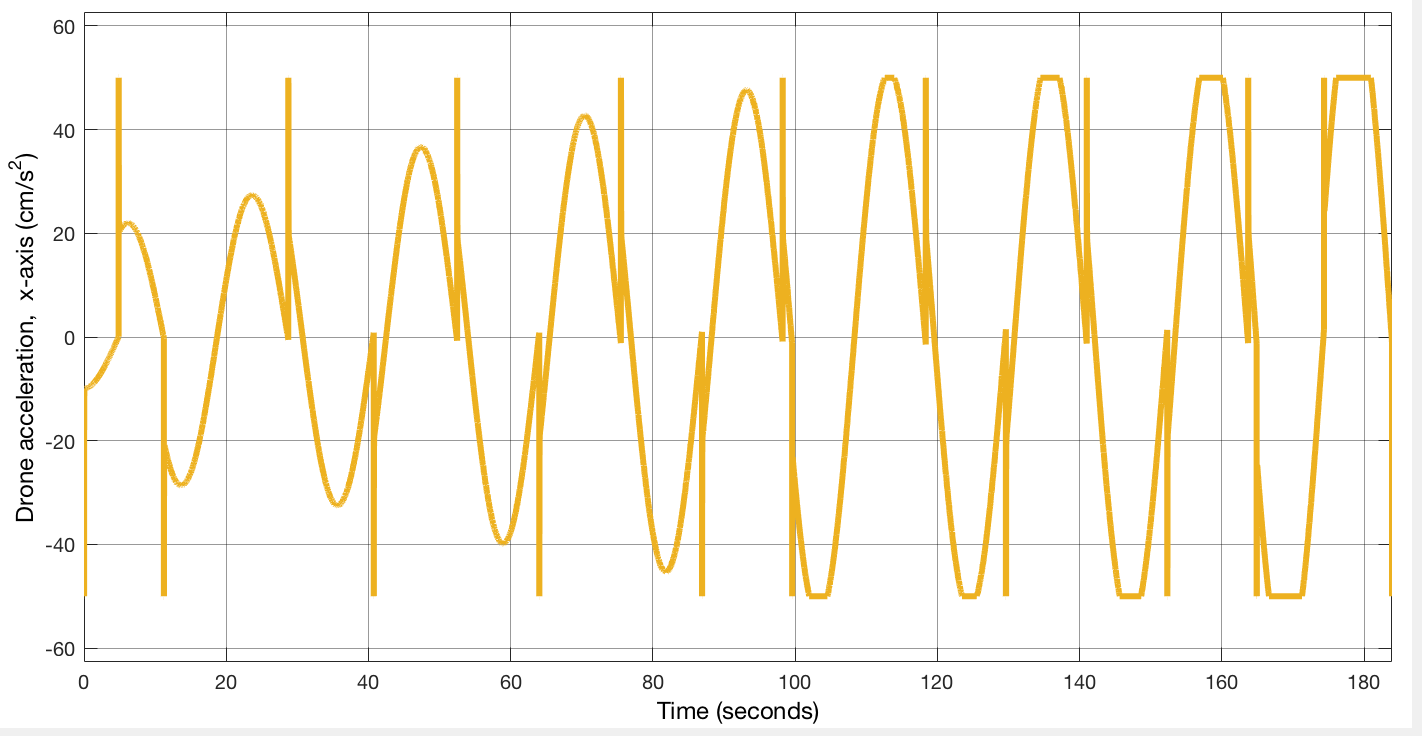
\includegraphics[width=.8\columnwidth]{figures/SA_accel_with_no_vel_limit.png}
  \caption{Acceleration of agent - without velocity limit}
  \label{fig:sa_accel_no_vel_adj}
\end{figure}






